\documentclass[conference]{IEEEtran}

\usepackage[T1]{fontenc}
\usepackage[utf8]{inputenc}
\usepackage{amsmath,amssymb}
\usepackage{booktabs}
\usepackage{array}
\usepackage{multirow}
\usepackage{tabularx}
\usepackage{adjustbox}
\usepackage{graphicx}
\usepackage{tikz}
\usetikzlibrary{arrows.meta,positioning,shapes.geometric}
\usepackage{url}
\usepackage[hidelinks]{hyperref}

\title{Fact Validator: A Transparent and Deployment-Ready Fact-Checking Architecture with Auditable Credibility Scoring, Tool-Augmented Evidence Retrieval, and Versioned 5000-Claim Evaluation}

\author{\IEEEauthorblockN{Author One, Author Two, Author Three}
\IEEEauthorblockA{Department of Computer Engineering\\
University of Naples Federico II\\
Naples, Italy\\
author1@example.com, author2@example.com, author3@example.com}}

\begin{document}

\maketitle

\begin{abstract}
Fact Validator is an end-to-end fact-checking architecture for misinformation risk assessment over free text and URL-derived content. The system decomposes input into claims, retrieves web evidence, applies an auditable domain-credibility prior, semantically reranks evidence, and aggregates claim-level verdicts into a final misinformation likelihood score. In contrast to purely model-centric factuality studies, this work contributes a deployment-ready research artifact with caching, persistence, health-aware fallbacks, and reproducible reporting. We evaluate the system on a frozen 5000-claim benchmark assembled from FEVER, LIAR, SciFact, and a normalized health-domain benchmark. On this versioned run, the default full pipeline reaches 50.82\% accuracy, exceeding the majority baseline by 1.56 percentage points and a length heuristic by 1.40 percentage points; the best frozen variant reaches 51.34\% without the debate layer, while the best tuned deployment-oriented variant reaches 50.98\%. Caching reduces estimated monthly evidence-retrieval cost by 71.43\%. Relative to Zero-shot Faithful Factual Error Correction and FacTool, the core novelty is not a universal claim of superior factuality, but a stronger integration of source-aware transparency, operational accountability, and deployment realism.
\end{abstract}

\begin{IEEEkeywords}
fact checking, misinformation detection, claim verification, credibility scoring, retrieval-augmented verification, explainable AI, benchmark evaluation
\end{IEEEkeywords}

\section{Introduction}

Automated fact checking is useful only if it can do more than emit a label. A practical system must surface evidence, express why it trusted one source more than another, remain robust when external services fail, and make its resource costs explicit. These requirements are often secondary in benchmark-driven factuality research, yet they are central in real deployment settings where misinformation analysis must be inspectable and reproducible.

Fact Validator was built around that gap. The project combines evidence retrieval, explicit source credibility scoring, optional debate arbitration, sentiment-aware risk adjustment, and persistent run storage in a full-stack application. The work is therefore positioned as a systems-and-methodology contribution: it aims to show how a fact-checking architecture can be made transparent, auditable, and operational at the same time.

This paper makes three bounded claims. First, Fact Validator provides a reproducible architecture for source-aware claim verification and misinformation likelihood scoring. Second, the repository contains a versioned 5000-claim evaluation pipeline that shows modest descriptive improvements over simple baselines in one frozen run. Third, the strongest contribution of the project remains architectural and methodological rather than a claim of state-of-the-art task performance.

\section{Related Work and Positioning}

\subsection{Zero-shot Faithful Factual Error Correction}

Zero-shot Faithful Factual Error Correction addresses a narrower problem than this project: it focuses on detecting and correcting factual errors without task-specific supervised retraining \cite{kubota2023zero}. Its strength is transferability across correction settings and its emphasis on preserving semantic faithfulness during rewriting. Fact Validator differs in both task definition and system boundary. Rather than rewriting single sentences, it verifies extracted claims against live web evidence and estimates misinformation likelihood for larger input content. As a result, the comparison is not primarily about raw correction quality. The stronger comparative statement is that Fact Validator extends the verification loop outward into retrieval, source scoring, persistence, and user-facing explanation.

\subsection{FacTool}

FacTool is the closer conceptual neighbor because it frames factuality checking as a tool-augmented pipeline \cite{grave2023factool}. That design principle is shared here: Fact Validator also relies on retrieval and external tools rather than trusting a single language model. The difference is where the additional value is placed. FacTool emphasizes modular factuality verification for generative AI outputs. Fact Validator emphasizes auditable domain credibility priors, persistent deployment, cost-aware caching, and full-stack operability for open-domain misinformation analysis. In other words, FacTool is a strong reference point for modular verification; Fact Validator pushes further on transparency of trust assignment and on production constraints.

\subsection{Comparative Research Position}

The comparison to both papers is therefore asymmetric. Fact Validator is not evaluated here against those systems on a shared benchmark with matched metrics. The argument is instead conceptual: this work places more explicit emphasis on source-trust modeling, persistence, cost-aware caching, and operational reporting within a deployable verification stack.

\section{System Architecture}

Fact Validator uses a nine-stage pipeline:

\begin{enumerate}
  \item content extraction from a URL or acceptance of raw text,
  \item claim decomposition into fact-like statements,
  \item web evidence retrieval through SerpAPI,
  \item source credibility scoring,
  \item semantic reranking of retrieved evidence,
  \item baseline verdict classification,
  \item optional LLM debate arbitration,
  \item sentiment and bias analysis,
  \item final misinformation scoring and persistence.
\end{enumerate}

\begin{figure}[t]
\centering
\resizebox{\columnwidth}{!}{%
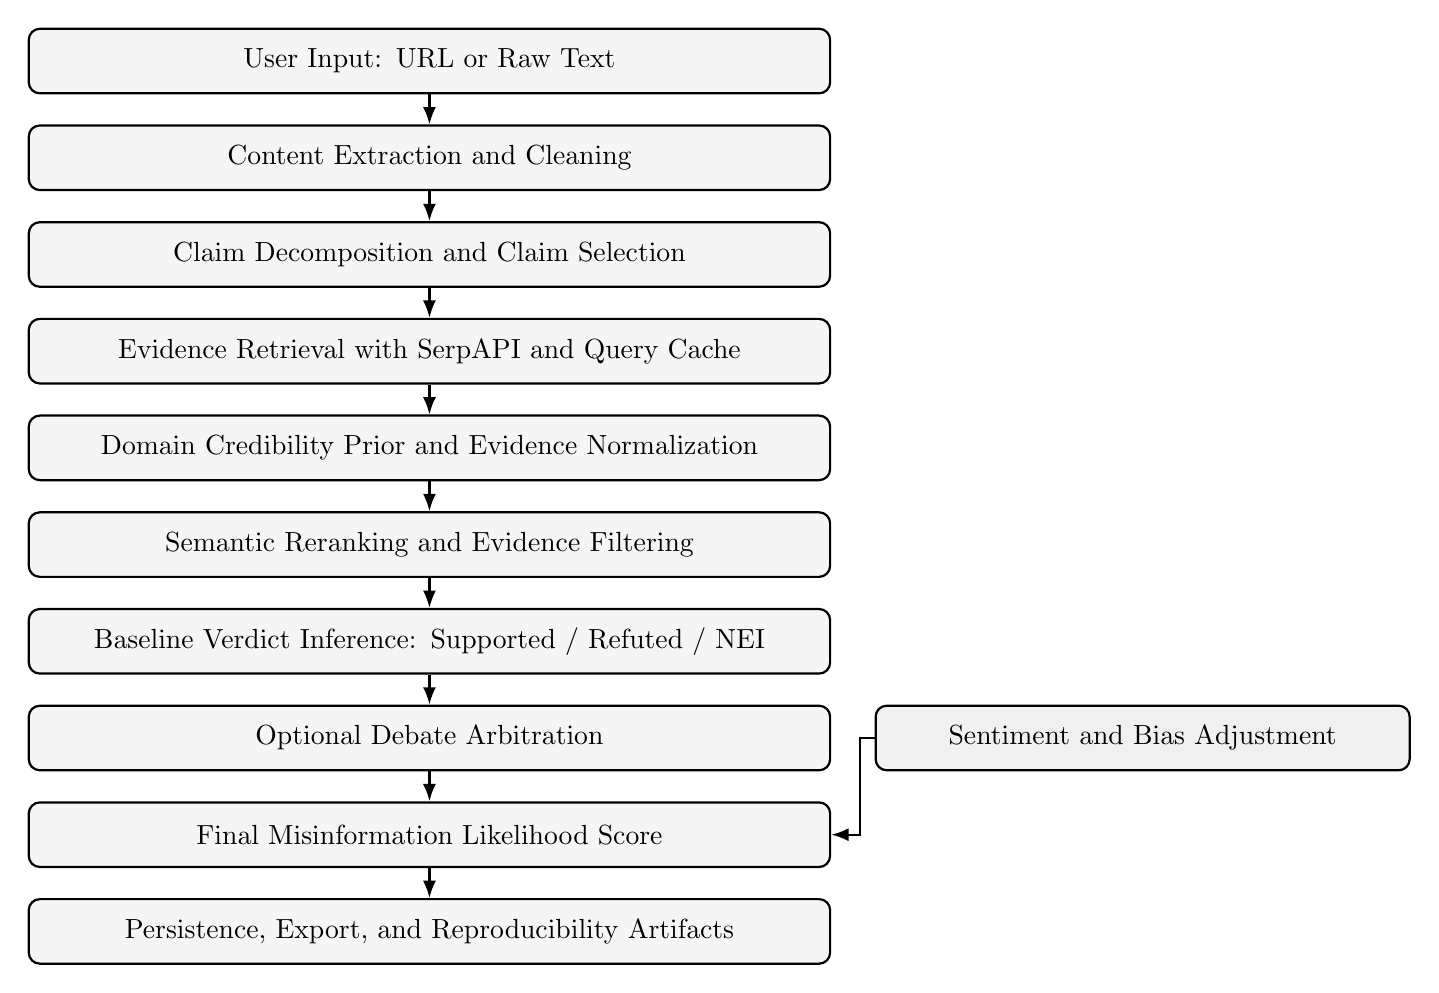
\begin{tikzpicture}[
  node distance=0.38cm,
  block/.style={rectangle, rounded corners, draw=black, thick, align=center, minimum height=0.82cm, text width=0.82\columnwidth, fill=gray!8},
  sideblock/.style={rectangle, rounded corners, draw=black, thick, align=center, minimum height=0.82cm, text width=0.54\columnwidth, fill=gray!12},
  line/.style={-{Latex[length=2.2mm]}, thick}
]
\node[block] (input) {User Input: URL or Raw Text};
\node[block, below=of input] (extract) {Content Extraction and Cleaning};
\node[block, below=of extract] (claims) {Claim Decomposition and Claim Selection};
\node[block, below=of claims] (retrieve) {Evidence Retrieval with SerpAPI and Query Cache};
\node[block, below=of retrieve] (credibility) {Domain Credibility Prior and Evidence Normalization};
\node[block, below=of credibility] (rerank) {Semantic Reranking and Evidence Filtering};
\node[block, below=of rerank] (verdict) {Baseline Verdict Inference: Supported / Refuted / NEI};
\node[block, below=of verdict] (debate) {Optional Debate Arbitration};
\node[sideblock, right=0.55cm of debate] (sentiment) {Sentiment and Bias Adjustment};
\node[block, below=of debate] (final) {Final Misinformation Likelihood Score};
\node[block, below=of final] (persist) {Persistence, Export, and Reproducibility Artifacts};

\draw[line] (input) -- (extract);
\draw[line] (extract) -- (claims);
\draw[line] (claims) -- (retrieve);
\draw[line] (retrieve) -- (credibility);
\draw[line] (credibility) -- (rerank);
\draw[line] (rerank) -- (verdict);
\draw[line] (verdict) -- (debate);
\draw[line] (debate) -- (final);
\draw[line] (sentiment.west) -- ++(-0.18,0) |- (final.east);
\draw[line] (final) -- (persist);
\end{tikzpicture}
}
\caption{End-to-end architecture of Fact Validator. The pipeline combines evidence retrieval, explicit credibility scoring, selective LLM arbitration, and persistent reporting in one auditable workflow.}
\label{fig:architecture}
\end{figure}

The client layer is implemented in Next.js, the orchestration layer in FastAPI, and the storage layer through SQLite plus JSON caches. The architecture is intentionally hybrid: rule-based and retrieval-based components are used where transparency matters most, while model-driven components are optional and isolated so that the system can degrade gracefully when an LLM service is unavailable.

Figure~\ref{fig:architecture} shows the publication-facing architecture view. The design separates deterministic evidence handling from optional LLM arbitration so that the system remains inspectable and can degrade gracefully when the debate service is unavailable.

\subsection{Auditable Credibility Scoring}

The credibility prior is explicit rather than learned:

\[
\mathrm{Score}(d) = \mathrm{clip}_{[0,100]}\bigl(50 + b(d) + p(d)\bigr)
\]

where $b(d)$ adds bonuses for recognized high-trust domains and $p(d)$ applies penalties for known low-trust or platform-style domains. This design improves interpretability because the source-trust mapping can be inspected, challenged, and modified without retraining the complete system.

\subsection{Operational Layer}

Caching is treated as a first-class research variable rather than an implementation detail. The system memoizes normalized claims with a 24-hour TTL and stores previous analyses for reproducibility. Structured persistence and fallback behavior are part of the contribution because they make large comparative runs feasible and auditable.

\section{Evaluation Protocol}

\subsection{Benchmark Family}

The strongest frozen evaluation surface in the repository is the versioned 5000-claim benchmark recorded in the 2026-07-02 result family. The benchmark is assembled from FEVER \cite{thorne2018fever}, LIAR \cite{wang2017liar}, SciFact \cite{wadden2020fact}, and a normalized health-domain dataset used in the healthver slot of the pipeline. The test split contains 5000 claims, with 11986 training claims and 2997 validation claims.

More precisely, the healthver slot was populated with the \texttt{health\_fact} dataset rather than the original HealthVer release. The import pipeline sampled 8000 FEVER v1.0 claims, 6000 LIAR claims, 1200 SciFact claims, and 6000 \texttt{health\_fact} claims, then deduplicated normalized claim text to retain 19983 unique claims before splitting. Exact textual duplicates were excluded across train, validation, and test partitions by withholding all normalized test claims from the remaining pool.

\begin{table}[htbp]
\centering
\caption{Benchmark composition and label harmonization.}
\label{tab:data}
\footnotesize
\setlength{\tabcolsep}{3pt}
\begin{adjustbox}{max width=\columnwidth}
\begin{tabular}{p{1.35cm}p{1.55cm}rrp{3.35cm}}
\toprule
Slot & Upstream source & Imported & Test $n$ & Canonical label mapping \\
\midrule
FEVER & FEVER v1.0 & 8000 & 1829 & SUPPORTS $\rightarrow$ SUPPORTED; REFUTES $\rightarrow$ REFUTED; NOT ENOUGH INFO $\rightarrow$ NEI \\
LIAR & LIAR & 6000 & 1490 & true, mostly-true $\rightarrow$ SUPPORTED; false, pants-fire $\rightarrow$ REFUTED; half-true, barely-true $\rightarrow$ NEI \\
SciFact & SciFact claims & 1200 & 191 & SUPPORT $\rightarrow$ SUPPORTED; CONTRADICT $\rightarrow$ REFUTED; empty label $\rightarrow$ NEI \\
healthver slot & health\_fact substitute & 6000 & 1490 & 2 $\rightarrow$ SUPPORTED; 0 $\rightarrow$ REFUTED; 1 and 3 $\rightarrow$ NEI \\
\bottomrule
\end{tabular}
\end{adjustbox}
\end{table}

The normalized CSV artifacts preserve source URLs and dataset identifiers but do not embed a complete license manifest. In the upstream dataset cards, FEVER is distributed under CC BY-SA 3.0 with additional Wikipedia-derived terms, SciFact is released under CC BY-NC 2.0, and the Hugging Face LIAR mirror marks licensing as unknown. The Health-Fact substitute used in the healthver slot should likewise be checked against its upstream dataset card before redistribution.

Claims and labels are frozen in the archived split files and result artifacts. Retrieved web evidence is not separately packaged as a static corpus, so exact replay should use the archived 2026-07-02 outputs rather than fresh live retrieval.

\subsection{Primary Systems Reported}

To avoid mixing incompatible result families, this paper reports only the frozen 5000-claim outputs. We focus on:

\begin{itemize}
  \item \textbf{Full Fact Validator} (internal artifact name: \texttt{full\_proxy}),
  \item \textbf{FEVER-aware exploratory variant} (internal artifact name: \texttt{tune\_fever}),
  \item \textbf{Fact Validator without debate} (internal artifact name: \texttt{ablate\_debate}),
  \item simple baselines: majority, length, random, keyword, and sentiment.
\end{itemize}

The FEVER-aware exploratory variant applies a fixed post-hoc margin adjustment to FEVER-labeled claims by increasing REFUTED and NEI scores inside the evaluation code. It is therefore reported as an exploratory dataset-aware variant rather than as a blind model-selection result.

\subsection{Metrics}

We report accuracy, macro-F1, average confidence, a simple confidence-accuracy gap, per-dataset deltas, and operational metrics for latency, throughput, and cost. In this paper version, paired significance tests are not reported; the comparisons are descriptive rather than inferential.

\section{Results}

Table~\ref{tab:main} summarizes the main benchmark results.

\begin{table}[htbp]
\centering
\caption{Main descriptive results on the frozen 5000-claim benchmark.}
\label{tab:main}
\footnotesize
\setlength{\tabcolsep}{3pt}
\begin{adjustbox}{max width=\columnwidth}
\begin{tabular}{lrrrrr}
\toprule
System & Accuracy & Macro-F1 & 95\% CI & Avg. Confidence & Conf.-Acc. Gap \\
\midrule
Fact Validator without debate & 0.5134 & 0.4427 & [0.4995, 0.5273] & 88.37 & 0.3703 \\
FEVER-aware exploratory variant & 0.5098 & 0.4421 & [0.4959, 0.5237] & 88.53 & 0.3755 \\
Full Fact Validator & 0.5082 & 0.4384 & [0.4943, 0.5221] & 88.31 & 0.3749 \\
Length heuristic & 0.4942 & 0.3483 & [0.4803, 0.5081] & 48.83 & 0.0059 \\
Majority baseline & 0.4926 & 0.2200 & [0.4787, 0.5065] & 50.00 & 0.0074 \\
Random baseline & 0.3320 & 0.3240 & [0.3189, 0.3451] & 50.00 & 0.1680 \\
Keyword heuristic & 0.2354 & 0.1364 & [0.2236, 0.2472] & 23.62 & 0.0008 \\
Sentiment heuristic & 0.2378 & 0.1400 & [0.2260, 0.2496] & 40.31 & 0.1653 \\
\bottomrule
\end{tabular}
\end{adjustbox}
\end{table}

The most important descriptive pattern is the performance of the full pipeline against the strongest simple baselines. In the frozen strict-validation snapshot, the full system exceeds the majority baseline by 1.56 percentage points and the length heuristic by 1.40 percentage points. No paired significance claim is made here because the paper does not report McNemar statistics, paired bootstrap intervals for the delta, or other inferential tests. The best observed variant in this frozen run is the debate-free ablation at 51.34\%, suggesting that debate should be treated as a selective inspection mechanism rather than as a universal default.

\begin{table}[htbp]
\centering
\caption{Per-dataset comparison for the default full pipeline from the strict-validation snapshot.}
\label{tab:dataset}
\footnotesize
\setlength{\tabcolsep}{4pt}
\begin{adjustbox}{max width=\columnwidth}
\begin{tabular}{lrrrrr}
\toprule
Dataset & $n$ & Full & Majority & Length & Full-Majority \\
\midrule
FEVER & 1829 & 0.5752 & 0.5856 & 0.5790 & -0.0104 \\
Health domain & 1490 & 0.5517 & 0.5154 & 0.5255 & +0.0362 \\
LIAR & 1490 & 0.3859 & 0.3658 & 0.3698 & +0.0201 \\
SciFact & 191 & 0.4817 & 0.4136 & 0.4084 & +0.0681 \\
\bottomrule
\end{tabular}
\end{adjustbox}
\end{table}

The per-dataset view matters more than the aggregate alone. The current system is strongest on SciFact and health-domain claims, positive on LIAR, and slightly negative on FEVER. That pattern supports a calibrated publication argument: the architecture is helpful for mixed-source, source-sensitive verification, but it still has distribution-specific weaknesses.

\section{Comparison to the Two Reference Papers}

Table~\ref{tab:comparepapers} summarizes the most useful comparison dimensions.

\begin{table*}[t]
\centering
\caption{Positioning relative to the two requested reference papers.}
\label{tab:comparepapers}
\footnotesize
\renewcommand{\arraystretch}{1.12}
\begin{tabularx}{\textwidth}{>{\raggedright\arraybackslash}p{2.2cm} >{\raggedright\arraybackslash}X >{\raggedright\arraybackslash}X >{\raggedright\arraybackslash}X}
\toprule
Dimension & Zero-shot Faithful Factual Error Correction & FacTool & Fact Validator \\
\midrule
Primary task & faithful error detection and correction & tool-augmented factuality detection & open-domain misinformation likelihood and claim verification \\
Evidence source & external knowledge for correction faithfulness & tool orchestration and retrieval modules & live web retrieval plus explicit domain-credibility priors \\
Transparency surface & faithful correction logic & modular tool use & auditable source scoring, stored runs, exportable evidence, explicit fallback behavior \\
Deployment emphasis & research method & research framework & full-stack application with persistence, caching, health checks, and cost tracking \\
Strongest advantage of Fact Validator & broader end-to-end verification workflow & stronger source-trust explicability and operational reporting & integrated architecture for practical deployment \\
\bottomrule
\end{tabularx}
\end{table*}

This comparison supports a conceptual, not empirical, distinction. Relative to the two selected reference works, Fact Validator places greater explicit emphasis on source-trust transparency, persistence, caching, and operational reporting. Direct superiority cannot be established without evaluating all systems on shared datasets and metrics.

\section{Novelty and Contribution}

The repository supports four publishable contributions.

\begin{enumerate}
  \item \textbf{Auditable source credibility as a first-class prior.} The system models source trust explicitly rather than burying it inside a learned verifier.
  \item \textbf{A full-stack fact-checking artifact.} The contribution is not only an algorithm but a working architecture spanning ingestion, verification, storage, and presentation.
  \item \textbf{Operational metrics in the evaluation loop.} The paper reports cost and latency alongside prediction quality, which is often omitted in fact-checking papers.
  \item \textbf{Versioned comparative benchmarking.} The project contains a reproducible external benchmark pipeline and stored run artifacts suitable for follow-up validation.
\end{enumerate}

\section{Discussion}

The 5000-claim result family shows a small observed gain over majority and length baselines together with substantial overconfidence. This profile is more consistent with a systems-and-methodology contribution than with a claim of universal model superiority.

The comparison to the two reference papers should therefore be read as complementary rather than adversarial. Zero-shot Faithful Factual Error Correction remains stronger on the sentence-level correction problem it directly targets. FacTool remains a clean framing of tool-augmented factuality analysis. Fact Validator's contribution is to show how those ideas can be operationalized in a source-aware, persistent, deployable verification stack.

\section{Limitations}

The strongest limitation is calibration. The full system is accurate enough to edge simple baselines on the frozen 5000-claim run, but its average confidence remains much higher than its observed accuracy. That means the system is useful as a decision-support pipeline, not as an unchecked automated adjudicator. Debate mode is another limitation: it adds complexity without helping the frozen benchmark when enabled by default. Finally, the health-domain portion of the benchmark uses a normalized substitute route, which should be documented carefully in any submission.

\section{Conclusion}

Fact Validator is best positioned as a transparent systems contribution for practical misinformation analysis. On the frozen 5000-claim benchmark family, the architecture delivers a modest observed edge over simple baselines while preserving evidence traceability and reproducibility. The broader scientific contribution is architectural: auditable source-trust modeling, persistent evidence workflows, and cost-aware deployment under realistic constraints. Relative to Zero-shot Faithful Factual Error Correction and FacTool, the project is most novel in how it operationalizes factuality research into a deployable and inspectable verification stack. Future work should focus on calibration improvements, evidence freezing for exact replay, broader external validation, and paired inferential testing for benchmark deltas.

\begin{thebibliography}{99}

\bibitem{kubota2023zero}
K.-H. Huang, H. P. Chan, and H. Ji, ``Zero-shot Faithful Factual Error Correction,'' \emph{arXiv preprint arXiv:2305.07982}, 2023.

\bibitem{grave2023factool}
I.-C. Chern, S. Chern, S. Chen, W. Yuan, K. Feng, C. Zhou, J. He, G. Neubig, and P. Liu, ``FacTool: Factuality Detection in Generative AI -- A Tool Augmented Framework for Multi-Task and Multi-Domain Scenarios,'' \emph{arXiv preprint arXiv:2307.13528}, 2023.

\bibitem{thorne2018fever}
J. Thorne, A. Vlachos, C. Christodoulopoulos, and A. Mittal, ``FEVER: a large-scale dataset for fact extraction and VERification,'' in \emph{Proc. NAACL-HLT}, 2018, pp. 809--819.

\bibitem{wang2017liar}
W. Y. Wang, ``LIAR, LIAR Pants on Fire: A New Benchmark Dataset for Fake News Detection,'' in \emph{Proc. ACL}, 2017, pp. 422--426.

\bibitem{wadden2020fact}
D. Wadden, S. Lin, K. Lo, L. L. Wang, M. van Zuylen, A. Cohan, and H. Hajishirzi, ``Fact or Fiction: Verifying Scientific Claims,'' in \emph{Proc. EMNLP}, 2020.

\bibitem{ji2023hallucination}
Z. Ji \emph{et al.}, ``Survey of Hallucination in Natural Language Generation,'' \emph{ACM Comput. Surveys}, vol. 55, no. 12, pp. 1--38, 2023.

\bibitem{wen2024abstention}
B. Wen \emph{et al.}, ``Know Your Limits: A Survey of Abstention in Large Language Models,'' \emph{arXiv preprint arXiv:2407.18418}, 2024.

\end{thebibliography}

\end{document}